
%(BEGIN_QUESTION)
% Copyright 2007, Tony R. Kuphaldt, released under the Creative Commons Attribution License (v 1.0)
% This means you may do almost anything with this work of mine, so long as you give me proper credit

Calculate the pressure at the discharge end of this pipe ($P_2$), assuming water as the fluid (with a mass density $\rho$ = 1005.5 kg/m³ ),  9.81 m/s² as the acceleration of gravity ($g$), and frictionless flow (no pressure loss due to friction):

$$\includegraphics[width=15.5cm]{i02978x01.eps}$$


\vskip 10pt

\noindent
{\bf Bernoulli's equation:}

$$z_1 \rho g + {v_1^2 \rho \over 2} + P_1 = z_2 \rho g + {v_2^2 \rho \over 2} + P_2$$

\underbar{file i02978}
%(END_QUESTION)





%(BEGIN_ANSWER)

$P_2$ = 0.776 MPa

%(END_ANSWER)





%(BEGIN_NOTES)

%INDEX% Physics, dynamic fluids: Bernoulli's equation

%(END_NOTES)


